% Бүлэг 2

\chapter{Системийн шинжилгээ ба загварчлал}
\label{Chapter2}

\section{Асуудлын тодорхойлолт}
\subsection{Одоогийн хэрэглэгдэж буй процесс, түүний хүндрэл, доголдол}

2026 оны байдлаар Монгол Улсын иргэд эрх зүйн туслалцаа авахдаа Legalinfo.mn, E-khutuch.mn зэрэг платформуудыг ашиглаж байгаа боловч дараах технологийн болон хэрэглээний хүндрэлүүд байсаар байна:

\begin{itemize}
    \item \textbf{Хайлтын механизмын хязгаарлагдмал байдал:} Одоогийн олон систем түлхүүр үгийн хайлт дээр суурилдаг тул хэрэглэгч хууль зүйн нарийн нэр томьёог мэдэхгүй үед холбогдох заалтыг олоход хүндрэлтэй байдаг.

    \item \textbf{Утга агуулгаар тайлбарлах боломж сул:} Хууль, эрх зүйн бичвэрүүд нь мэргэжлийн хэллэг, нарийн бүтэцтэй тул энгийн хэрэглэгч уншаад өөрийн нөхцөл байдалд хэрхэн хамаарахыг ойлгоход төвөгтэй байдаг.

    \item \textbf{Мэдээллийн тархай бутархай байдал:} Эрүүгийн, Иргэний, Захиргааны, Хөдөлмөрийн зэрэг олон төрлийн хууль, түүнтэй холбоотой тайлбар, журам, эх сурвалжууд салангид байрладаг тул хэрэглэгч нэг дороос цогц ойлголт авахад хүндрэл учирдаг.

    \item \textbf{Анхан шатны зөвлөгөө авах хүртээмж сул:} Энгийн хэрэглэгчид хуульчид шууд хандахаас өмнө анхан шатны, ойлгомжтой, бодит эх сурвалжид суурилсан зөвлөгөө авах дижитал шийдэл хангалтгүй байна.

    \item \textbf{Харилцан ярианы түүхийн уялдаа муу:} Хэрэглэгч өмнөх асуулт, хариултаа хадгалж, тухайн кейсээ үргэлжлүүлэн лавшруулан асуух боломж олон системд хязгаарлагдмал байдаг.
\end{itemize}

\subsection{Хэрэглэгчдийн тулгамдсан асуудал}

\begin{itemize}
    \item \textbf{Буруу эсвэл үндэслэлгүй AI хариултын эрсдэл:} Ерөнхий зориулалтын AI хэрэгслүүдийг шууд ашиглах үед Монгол Улсын хууль, эрх зүйн орчинд тохироогүй, эсвэл бодит эх сурвалжгүй тайлбар өгөх эрсдэлтэй.

    \item \textbf{Цаг хугацаа ба зардал:} Энгийн асуултад хариулт авахын тулд заавал хуульчид хандах шаардлага үүсч, хугацаа болон зардал нэмэгддэг.

    \item \textbf{Ойлгомжгүй хууль зүйн хэллэг:} Хэрэглэгч хуулийн заалтыг олсон ч түүний агуулгыг өөрийн нөхцөл байдалтай холбон ойлгоход хэцүү байдаг.

    \item \textbf{Кейсийн мэдээлэл дахин дахин тайлбарлах шаардлага:} Хэрэглэгч асуултаа үргэлжлүүлэн тодруулах бүрд өмнөх мэдээллээ дахин оруулах хэрэгцээ гардаг.
\end{itemize}

%-------------------------------------------------------------------------------

\section{Хэрэглэгчийн шаардлагын шинжилгээ}
\subsection{Хэрэглэгчийн функциональ шаардлага}

Хууль зүйн зөвлөх системийн оролцогч талуудын шаардлагыг системийн үндсэн зорилго, хэрэглээний онцлогтой уялдуулан тодорхойлов. Систем нь зөвхөн эрүүгийн хуульд хязгаарлагдахгүй бөгөөд төрөл бүрийн хууль, эрх зүйн эх сурвалжид тулгуурлан хэрэглэгчид зөвлөгөө өгөх боломжтойгоор төлөвлөгдсөн.

\subsection{Хэрэглэгчийн үүрэг, ашиглалтын хувилбарууд}

\begin{enumerate}
    \item \textbf{Ерөнхий хэрэглэгч (Иргэн) -- ``Зөвлөгөө авах''}
    \begin{itemize}
        \item \textbf{AI-аас анхан шатны хууль зүйн зөвлөгөө авах:} Хэрэглэгч өөрт тулгарсан асуудлыг энгийн хэлээр оруулах бөгөөд систем нь өгөгдлийн сангаас холбогдох хууль, эрх зүйн зүйл заалтуудыг хайж, тэдгээрт тулгуурлан Google Gemini 2.5 Flash загвараар ойлгомжтой тайлбар бүхий хариулт боловсруулна.

        \item \textbf{Эх сурвалж баталгаажуулах:} AI-ийн гаргасан хариултын хамт холбогдох хууль, зүйл заалтын мэдээллийг харуулж, хэрэглэгч өөрөө шалган баталгаажуулах боломжтой.

        \item \textbf{Чат болон кейсийн түүх харах:} Хэрэглэгчийн асуулт, AI-ийн хариултыг кейс байдлаар хадгалсан мэдээллийг дараа нь дахин харах, үргэлжлүүлэн асуух боломжтой.

        \item \textbf{Профайл удирдах:} Хэрэглэгч өөрийн бүртгэлийн мэдээллээ шинэчлэх боломжтой.
    \end{itemize}

    \item \textbf{Мэргэжлийн хуульч (Lawyer) -- ``Мэргэжлийн шинжилгээ''}
    \begin{itemize}
        \item \textbf{Кейсийн хүрээнд хууль зүйн дүн шинжилгээ хийх:} Хуульч тухайн асуудалд холбогдох хууль, заалтыг системээс шүүж авч, AI-ийн тусламжтайгаар тайлбар, дүгнэлт боловсруулах боломжтой.

        \item \textbf{Баримт бичгийн боловсруулалт:} PDF хэлбэрийн хууль, эрх зүйн болон холбогдох баримт бичгээс текст задлан авч, системд оруулан боловсруулалт хийх боломжтой.

        \item \textbf{AI зөвлөх ашиглах:} Google Gemini 2.5 Flash загвараар кейсийн нөхцөл байдалд тулгуурласан нэмэлт тайлбар, анхаарах асуудал, боломжит хувилбаруудыг гаргаж болно.
    \end{itemize}

    \item \textbf{Админ (Admin) -- ``Системийн удирдлага''}
    \begin{itemize}
        \item \textbf{Хуулийн сан удирдах:} Шинэ хууль, эрх зүйн баримт бичгийг системд оруулж, боловсруулан өгөгдлийн санд хадгалах.

        \item \textbf{Хэрэглэгчийн эрх удирдах:} Хэрэглэгчийн бүртгэл, эрхийн түвшин, систем ашиглах боломжийг хянах.

        \item \textbf{Өгөгдлийн шинэчлэлт хийх:} Хуулийн ангилал, зүйл заалт, системийн агуулгыг шинэчлэх.
    \end{itemize}
\end{enumerate}

%-------------------------------------------------------------------------------

\section{Функционал бус шаардлага}

\subsection{Гүйцэтгэлийн шаардлага}

\begin{itemize}
    \item \textbf{Хариу өгөх хугацаа:} Backend болон AI боловсруулалтын нийлбэр хугацаа хэвийн нөхцөлд 3--8 секундээс хэтрэхгүй байх.

    \item \textbf{Нэгэн зэрэг хэрэглэгч боловсруулах чадвар:} Систем нь олон хэрэглэгчийн хүсэлтийг тогтвортой боловсруулах боломжтой байх.

    \item \textbf{Өргөтгөх боломж:} FastAPI болон PostgreSQL архитектур нь системийг цаашид шинэ төрлийн хууль, нэмэлт модуль, олон хэрэглэгчийн ачаалалд нийцүүлэн өргөтгөхөд тохиромжтой байх.

    \item \textbf{Төхөөрөмжийн нийцтэй байдал:} Frontend нь компьютер болон мобайл төхөөрөмж дээр зохистой ажиллах шаардлагатай.
\end{itemize}

\subsection{Аюулгүй байдлын шаардлага}

\begin{itemize}
    \item \textbf{Authentication:} Хэрэглэгчийн баталгаажуулалтыг JWT технологид суурилан хэрэгжүүлсэн байх.

    \item \textbf{Password Security:} Нууц үгийг bcrypt ашиглан hash хэлбэрээр хадгалдаг байх.

    \item \textbf{Access Control:} Хэрэглэгч, хуульч, админ зэрэг эрхийн түвшнүүдийг ялган хянах боломжтой байх.

    \item \textbf{Data Isolation:} Хэрэглэгч бүрийн кейс болон мессежийн өгөгдлийг тусгаарлан хадгалдаг байх.
\end{itemize}

\subsection{Хамгаалалт, нууцлалын шаардлага}

\begin{itemize}
    \item \textbf{Encrypted Communication:} Frontend болон backend хооронд өгөгдөл дамжуулахдаа хамгаалалттай холболт ашиглах.

    \item \textbf{Нууц түлхүүр болон тохиргооны хамгаалалт:} API key, database URL зэрэг системийн чухал тохиргоог орчны хувьсагчаар удирдах.

    \item \textbf{Хэрэглэгчийн мэдээллийн нууцлал:} Хэрэглэгчийн профайл, чат түүх, кейсийн мэдээллийг зөвшөөрөлгүй этгээдэд ил болгохгүй байх.
\end{itemize}

%-------------------------------------------------------------------------------

\section{Юзкейс диаграм ба хүснэгтэн тодорхойлолт}

Системийн гурван үндсэн оролцогч тал болох ерөнхий хэрэглэгч, хуульч, админ нарын ашиглалтын хувилбаруудыг дараах юзкейс диаграммуудаар дүрсэллээ.

\begin{figure}[H]
    \centering
    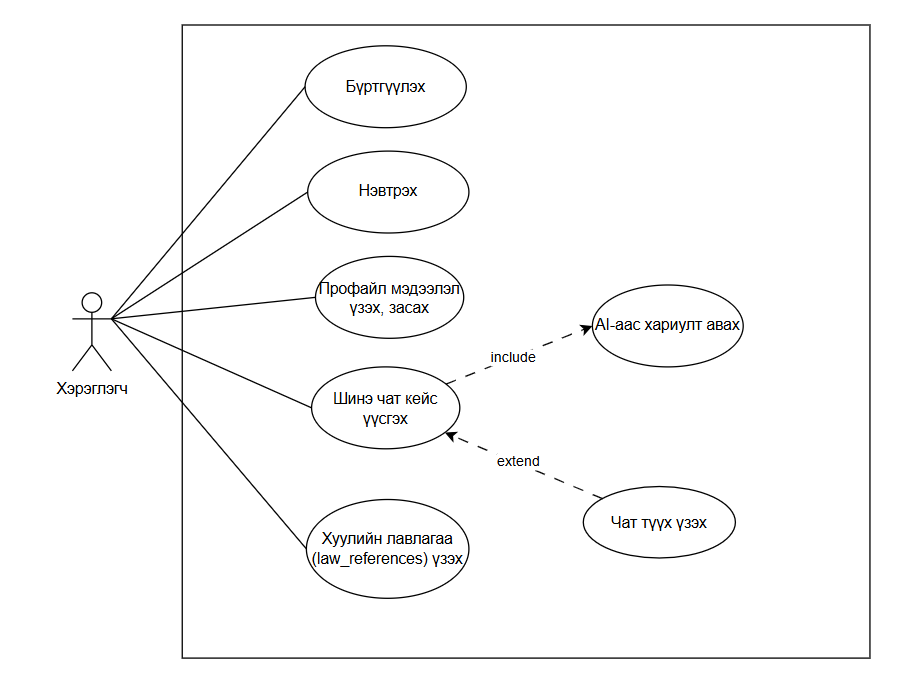
\includegraphics[width=\textwidth]{Diagrams/UsecaseUser.png}
    \caption[Юзкейс диаграм -- Хэрэглэгч]{Ерөнхий хэрэглэгчийн юзкейс диаграм}
    \label{fig:UseCaseUser}
\end{figure}

\noindent
Ерөнхий хэрэглэгч нь системд бүртгүүлж нэвтэрсний дараа чат интерфэйсэр асуулт оруулах, AI-аас хариулт авах, чат болон кейсийн түүхээ харах, профайл мэдээллээ удирдах зэрэг үндсэн үйлдлүүдийг гүйцэтгэнэ.

\begin{figure}[H]
    \centering
    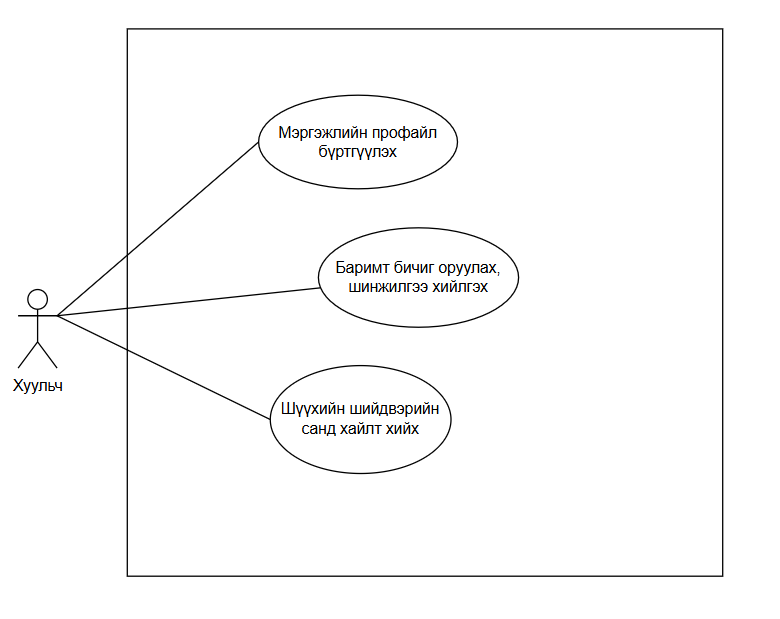
\includegraphics[width=\textwidth]{Diagrams/UsecaseLawyer.png}
    \caption[Юзкейс диаграм -- Хуульч]{Хуульчийн юзкейс диаграм}
    \label{fig:UseCaseLawyer}
\end{figure}

\noindent
Хуульч нь ерөнхий хэрэглэгчийн эрхээс гадна PDF баримт бичиг оруулж шинжилгээ хийлгэх, кейсийн хүрээнд нарийвчилсан дүн шинжилгээ авах боломжтой.

\begin{figure}[H]
    \centering
    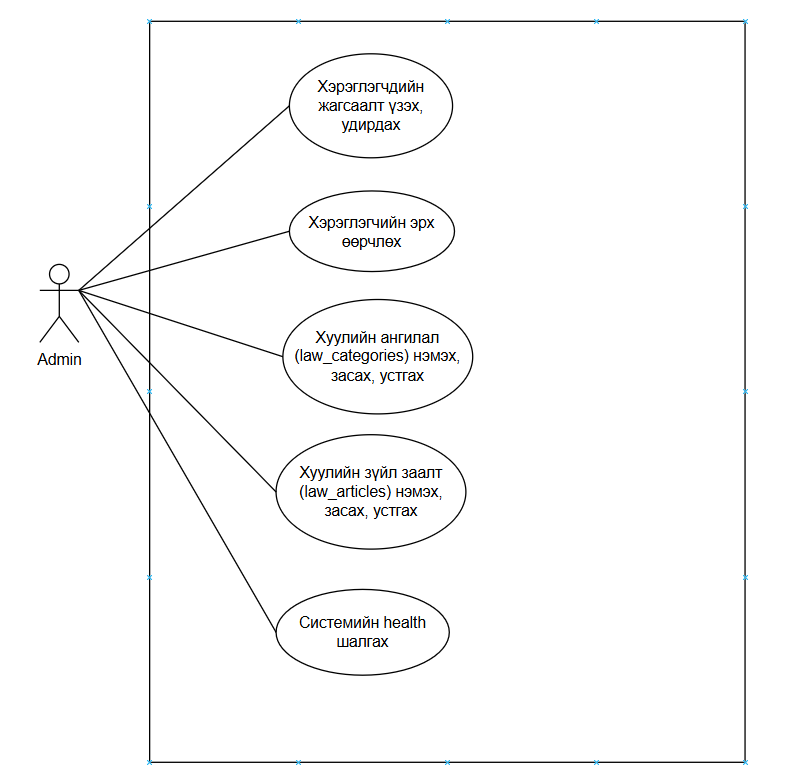
\includegraphics[width=\textwidth]{Diagrams/UsecaseAdmin.png}
    \caption[Юзкейс диаграм -- Админ]{Админий юзкейс диаграм}
    \label{fig:UseCaseAdmin}
\end{figure}

\noindent
Админ нь хуулийн санг шинэчлэх, хэрэглэгчийн эрх удирдах, системийн ерөнхий ажиллагааг хянах бүрэн эрхтэй.

\vspace{0.5cm}

\begin{table}[H]
\centering
\renewcommand{\arraystretch}{1.3}
\begin{tabular}{|p{3cm}|p{11cm}|}
\hline
\textbf{Юзкейс нэр} & AI-аас хууль зүйн зөвлөгөө авах \\ \hline
\textbf{Actor} & Ерөнхий хэрэглэгч (Иргэн) \\ \hline
\textbf{Зорилго} & Хэрэглэгчийн асуултад бодит эх сурвалжид тулгуурласан хууль зүйн зөвлөгөө өгөх \\ \hline
\textbf{Урьдчилсан нөхцөл} & Хэрэглэгч системд нэвтэрсэн байх, PostgreSQL өгөгдлийн сан болон AI үйлчилгээ ажиллах боломжтой байх \\ \hline
\textbf{Үндсэн урсгал} & \begin{minipage}[t]{11cm}
\begin{enumerate}
    \item Хэрэглэгч чат хэсэгт өөрт тулгарсан асуудлыг энгийн хэлээр бичнэ
    \item Систем backend түвшинд асуулгыг хүлээн авч боловсруулна
    \item PostgreSQL өгөгдлийн сангаас холбогдох хууль, зүйл заалтыг хайж олно
    \item Олдсон хууль зүйн мэдээлэл болон хэрэглэгчийн асуултыг нэгтгэн prompt үүсгэнэ
    \item Prompt-ийг Google Gemini 2.5 Flash загвар руу илгээнэ
    \item AI боловсруулсан хариултыг систем буцаан хүлээн авна
    \item Хариултыг чат түүхэнд хадгалж, хэрэглэгчийн дэлгэцэнд харуулна
\end{enumerate}
\end{minipage} \\ \hline
\textbf{Төгсгөл нөхцөл} & Хариулт хэрэглэгчийн дэлгэцэнд харагдаж, кейсийн түүхэнд хадгалагдсан байна \\ \hline
\end{tabular}
\caption{AI-аас хууль зүйн зөвлөгөө авах юзкейс}
\end{table}

\vspace{0.5cm}

\begin{table}[H]
\centering
\renewcommand{\arraystretch}{1.3}
\begin{tabular}{|p{3cm}|p{11cm}|}
\hline
\textbf{Юзкейс нэр} & Баримт бичгийн дүн шинжилгээ \\ \hline
\textbf{Actor} & Хуульч \\ \hline
\textbf{Зорилго} & Баримт бичгээс чухал агуулга, холбогдох хууль зүйн мэдээллийг ялган боловсруулах \\ \hline
\textbf{Урьдчилсан нөхцөл} & Хуульч системд зохих эрхтэйгээр нэвтэрсэн байх \\ \hline
\textbf{Үндсэн урсгал} & \begin{minipage}[t]{11cm}
\begin{enumerate}
    \item Хуульч PDF баримт бичгийг системд оруулна
    \item Систем PyMuPDF ашиглан баримт бичгээс текст задлан авна
    \item Текстийг боловсруулж, гол агуулга болон хууль зүйн холбогдох хэсгүүдийг ялгана
    \item Хуульч асуулт асуух үед backend нь баримтын агуулга болон өгөгдлийн сан дахь хууль зүйн мэдээллийг нэгтгэнэ
    \item Google Gemini 2.5 Flash ашиглан дүн шинжилгээ хийж, тайлбарласан хариулт гаргана
\end{enumerate}
\end{minipage} \\ \hline
\textbf{Төгсгөл нөхцөл} & Баримтын шинжилгээний үр дүн хэрэглэгчид харагдаж, шаардлагатай тохиолдолд хадгалагдсан байна \\ \hline
\end{tabular}
\caption{Баримт бичгийн дүн шинжилгээ юзкейс}
\end{table}

\vspace{0.5cm}

\begin{table}[H]
\centering
\renewcommand{\arraystretch}{1.3}
\begin{tabular}{|p{3cm}|p{11cm}|}
\hline
\textbf{Юзкейс нэр} & Хуулийн санг шинэчлэх \\ \hline
\textbf{Actor} & Админ \\ \hline
\textbf{Зорилго} & Шинэ хууль, эрх зүйн баримт бичгийг системд нэмэх, шинэчлэх \\ \hline
\textbf{Урьдчилсан нөхцөл} & Шинэ хууль, эрх зүйн эх сурвалж бэлэн болсон байх \\ \hline
\textbf{Үндсэн урсгал} & \begin{minipage}[t]{11cm}
\begin{enumerate}
    \item Админ шинэ хууль, эрх зүйн баримт бичгийг системд оруулна
    \item Систем баримтаас текстийг задлан авч боловсруулна
    \item Хуулийн ангилал, зүйл, заалт, дэд заалтыг ялгаж бүтэцжүүлнэ
    \item Боловсруулсан өгөгдлийг PostgreSQL өгөгдлийн санд хадгална
    \item Систем шинэчлэгдсэн өгөгдөлд тулгуурлан хэрэглэгчийн асуултад хариу өгөх боломжтой болно
\end{enumerate}
\end{minipage} \\ \hline
\textbf{Төгсгөл нөхцөл} & Шинэ хууль, эрх зүйн мэдээлэл системд амжилттай нэмэгдсэн байна \\ \hline
\end{tabular}
\caption{Хуулийн санг шинэчлэх юзкейс}
\end{table}

%-------------------------------------------------------------------------------

\section{Үйл ажиллагааны диаграм}

Систем нь хэрэглэгчийн нэвтрэлтийн үе шат болон чат хийх үе шат гэсэн хоёр үндсэн үйл явцаас бүрдэнэ. Эдгээр хоёр үйл явцыг тус тусад нь activity diagram хэлбэрээр дүрслэв.

\begin{figure}[H]
    \centering
    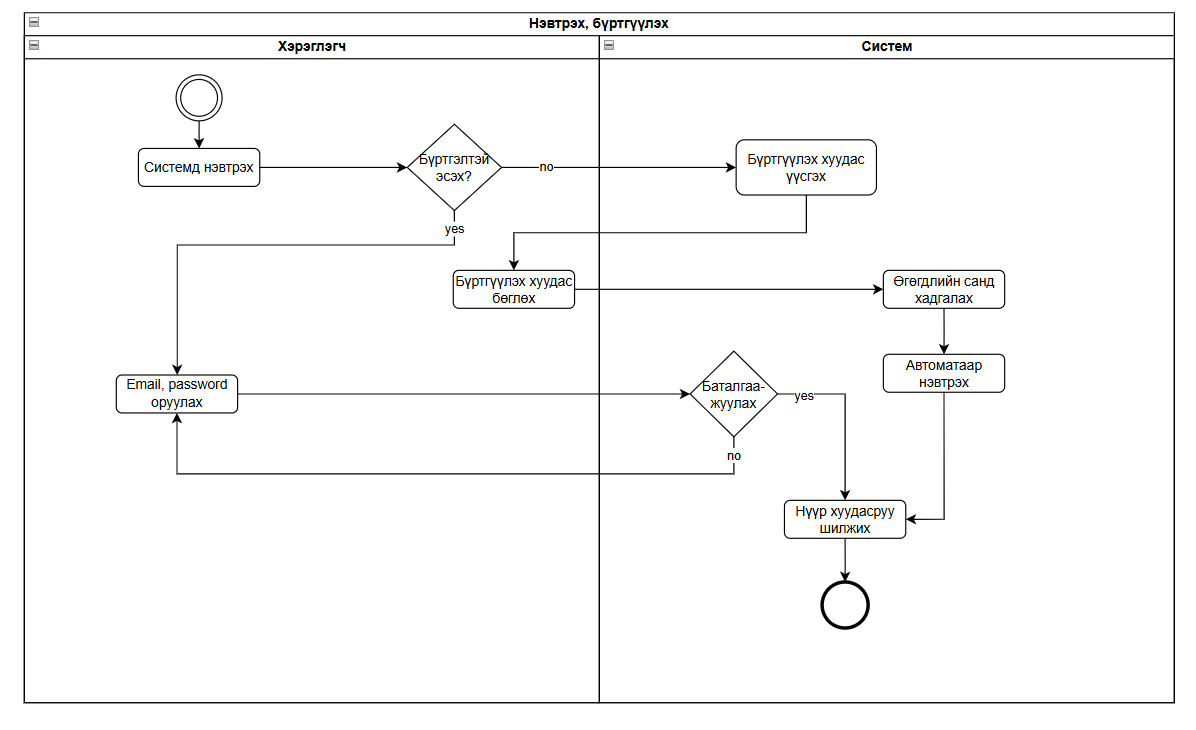
\includegraphics[width=\textwidth]{Diagrams/ActivityDiagramLogin.png}
    \caption[Нэвтрэлтийн үйл ажиллагааны диаграм]{Нэвтрэлтийн үйл ажиллагааны диаграм}
    \label{fig:ActivityDiagramLogin}
\end{figure}

\noindent
Нэвтрэлтийн диаграмм нь хэрэглэгч системд нэвтрэх хүсэлт илгээхээс эхлэн JWT токен амжилттай үүсэж хэрэглэгч системд орох хүртэлх бүх үе шатыг харуулна. Нэвтрэлт амжилтгүй болвол алдааны мессеж харуулж, хэрэглэгч дахин оролдох боломжтой байна.

\begin{figure}[H]
    \centering
    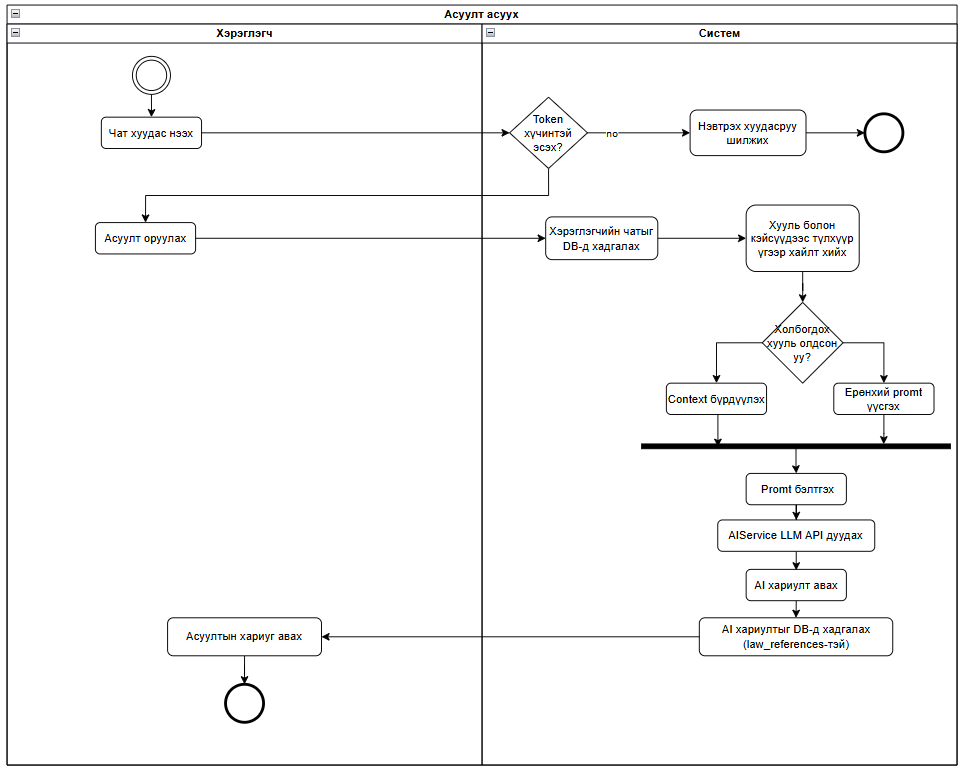
\includegraphics[width=\textwidth]{Diagrams/ActivityDiagramChat.png}
    \caption[Чатын үйл ажиллагааны диаграм]{Чатын үйл ажиллагааны диаграм}
    \label{fig:ActivityDiagramChat}
\end{figure}

\noindent
Чатын диаграмм нь хэрэглэгч асуулт оруулсан цагаасаа эхлэн RAG зарчмаар хуулийн мэдээлэл хайгдаж, Google Gemini 2.5 Flash загвараар хариулт боловсруулагдан хэрэглэгчид харуулагдах хүртэлх дэлгэрэнгүй урсгалыг дүрсэлнэ.

%-------------------------------------------------------------------------------

\section{Дарааллын диаграм}

Систем нь хэрэглэгчийн нэвтрэх болон хууль зүйн зөвлөгөө авах гэсэн хоёр үндсэн хэрэглээний хувилбартай бөгөөд тэдгээрийн объектуудын цагийн дарааллыг дараах диаграммуудаар харуулав.

\begin{figure}[H]
    \centering
    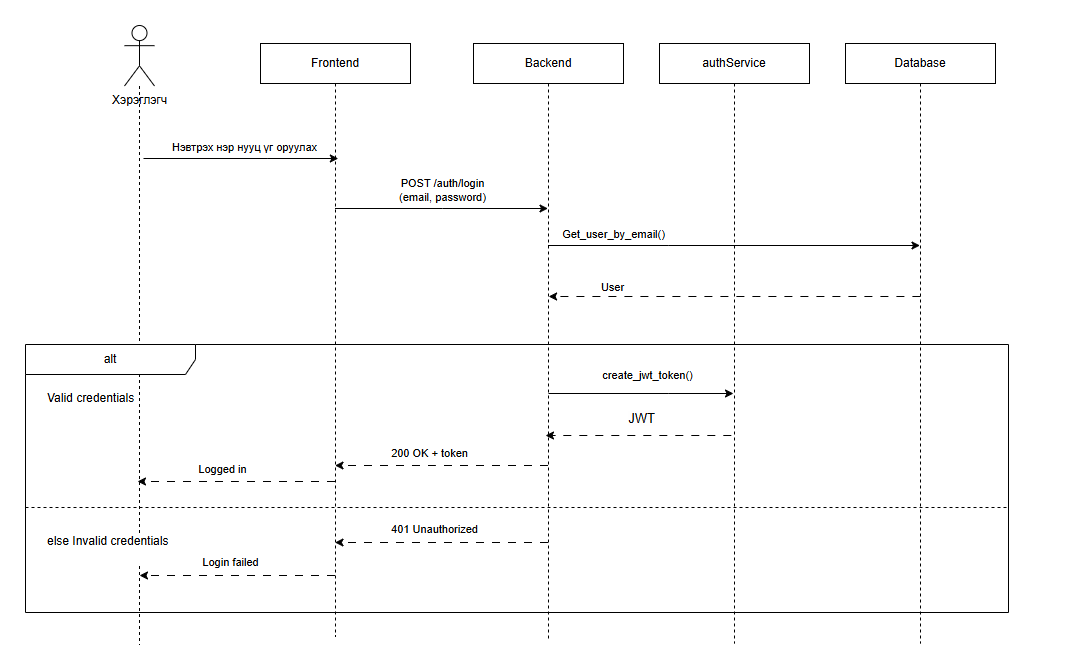
\includegraphics[width=\textwidth]{Diagrams/SequenceLogin.png}
    \caption[Нэвтрэлтийн дарааллын диаграм]{Нэвтрэлтийн дарааллын диаграм}
    \label{fig:SequenceLogin}
\end{figure}

\noindent
Нэвтрэлтийн дарааллын диаграмм нь хэрэглэгч нэвтрэх хүсэлт илгээснээс эхлэн Frontend $\rightarrow$ Backend $\rightarrow$ PostgreSQL гэсэн дарааллаар нэвтрэлт шалгагдаж, JWT токен үүсгэгдэн хэрэглэгчид буцаах үйл явцыг нарийвчлан харуулна.

\begin{figure}[H]
    \centering
    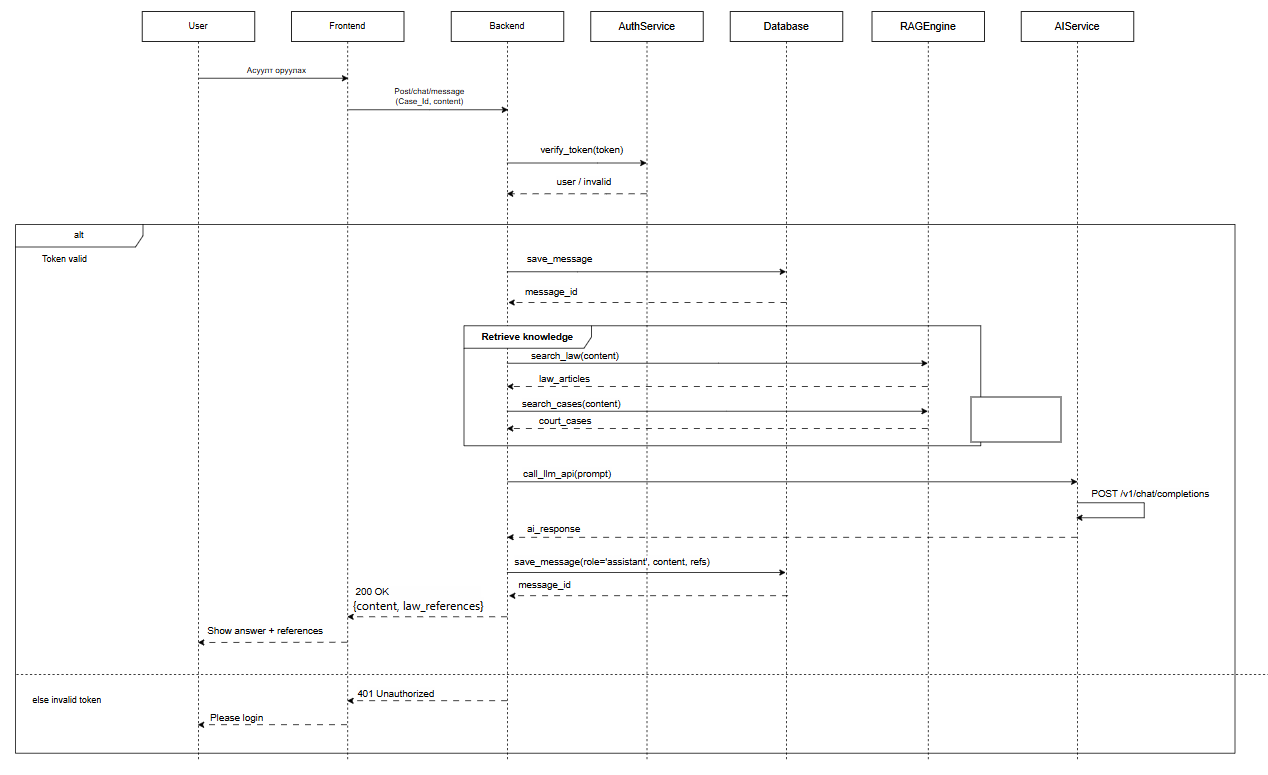
\includegraphics[width=\textwidth]{Diagrams/SequenceSystem.png}
    \caption[Системийн дарааллын диаграм]{Хууль зүйн зөвлөгөө авах дарааллын диаграм}
    \label{fig:SequenceSystem}
\end{figure}

\noindent
Системийн дарааллын диаграмм нь хэрэглэгчийн асуулга Frontend-ээс Backend рүү дамжин, Backend нь PostgreSQL өгөгдлийн сангаас холбогдох хууль, эрх зүйн мэдээллийг RAG зарчмаар хайж олсны дараа тухайн мэдээллийг хэрэглэгчийн асуулттай нэгтгэн Google Gemini 2.5 Flash загварт илгээж хариулт боловсруулах үйл явцыг харуулна. AI загвараас боловсруулсан хариулт буцаж ирсний дараа систем нь тухайн кейс болон мессежийн түүхийг өгөгдлийн санд хадгалж, эцсийн хариуг хэрэглэгчийн интерфэйс дээр харуулдаг.

%-------------------------------------------------------------------------------

\section{Хамаарлын диаграм}

\begin{figure}[H]
    \centering
    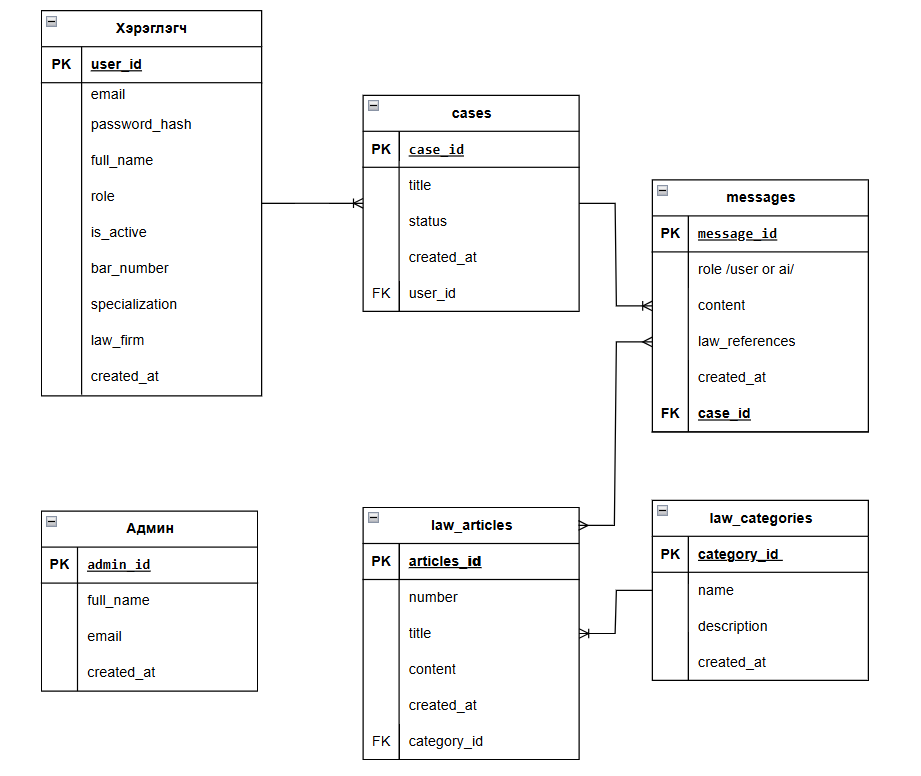
\includegraphics[width=\textwidth]{Diagrams/ERD.png}
    \caption[Хамаарлын диаграм]{Хамаарлын диаграм (Entity--Relationship Diagram, ERD)}
    \label{fig:ERD}
\end{figure}

\noindent
Хамаарлын диаграмм нь системийн үндсэн өгөгдлийн бүтэц болох хэрэглэгч (\texttt{users}), кейс (\texttt{cases}), мессеж (\texttt{messages}), хуулийн ангилал (\texttt{law\_categories}), хуулийн зүйл заалт (\texttt{law\_articles}) хоорондын хамаарлыг харуулна. Нэг хэрэглэгч олон кейстэй, нэг кейс олон мессежтэй холбогддог бөгөөд хуулийн өгөгдөл нь RAG зарчмаар хариулт боловсруулахад контекст болж ашиглагдана. Энэхүү бүтэц нь хэрэглэгчийн харилцан ярианы түүх болон хууль, эрх зүйн мэдээллийг нэгдсэн байдлаар удирдах боломжийг бүрдүүлдэг.

%-------------------------------------------------------------------------------

\section{Класс диаграм}

\begin{figure}[H]
    \centering
    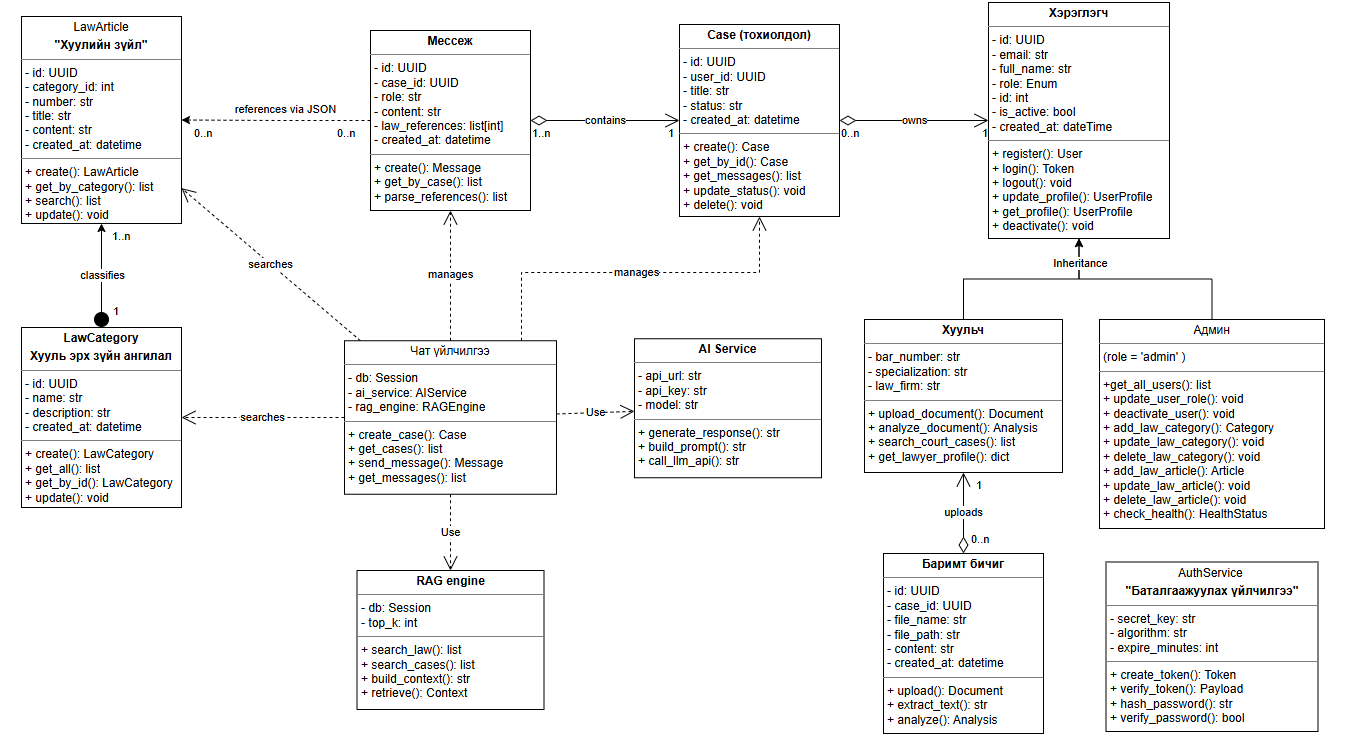
\includegraphics[width=\textwidth]{Diagrams/ClassDiagram.png}
    \caption[Класс диаграм]{Класс диаграм}
    \label{fig:ClassDiagram}
\end{figure}

\noindent
Класс диаграмм нь backend системийн үндсэн обьектууд болон тэдгээрийн хоорондын уялдаа холбоог дүрсэлнэ. Үүнд хэрэглэгч, профайл, кейс, мессеж, хуулийн ангилал, хуулийн зүйл заалт зэрэг entity-үүд болон тэдгээртэй ажиллах service, schema, route түвшний логик багтана. \textbf{User}, \textbf{Lawyer}, \textbf{Admin} классууд өөр өөрийн үүрэг, атрибуттай бөгөөд \textbf{Case} класс олон \textbf{Message}-тэй холбогдоно. \textbf{RAGEngine} класс нь хуулийн өгөгдлийг хайж олох болон prompt бүрдүүлэх үндсэн логикийг агуулна.

%-------------------------------------------------------------------------------

\section{Архитектурын шийдэл}

LexNavigator систем нь орчин үеийн веб технологид суурилсан, давхаргат (layered) болон модульчлагдсан (modular) архитектуртай систем юм. Энэхүү архитектур нь системийн бүрэлдэхүүн хэсгүүдийг үүргээр нь ялган зохион байгуулж, хөгжүүлэлт, өргөтгөл, засвар үйлчилгээ болон гүйцэтгэлийн үр ашгийг нэмэгдүүлэх зорилготой.

\begin{figure}[H]
    \centering
    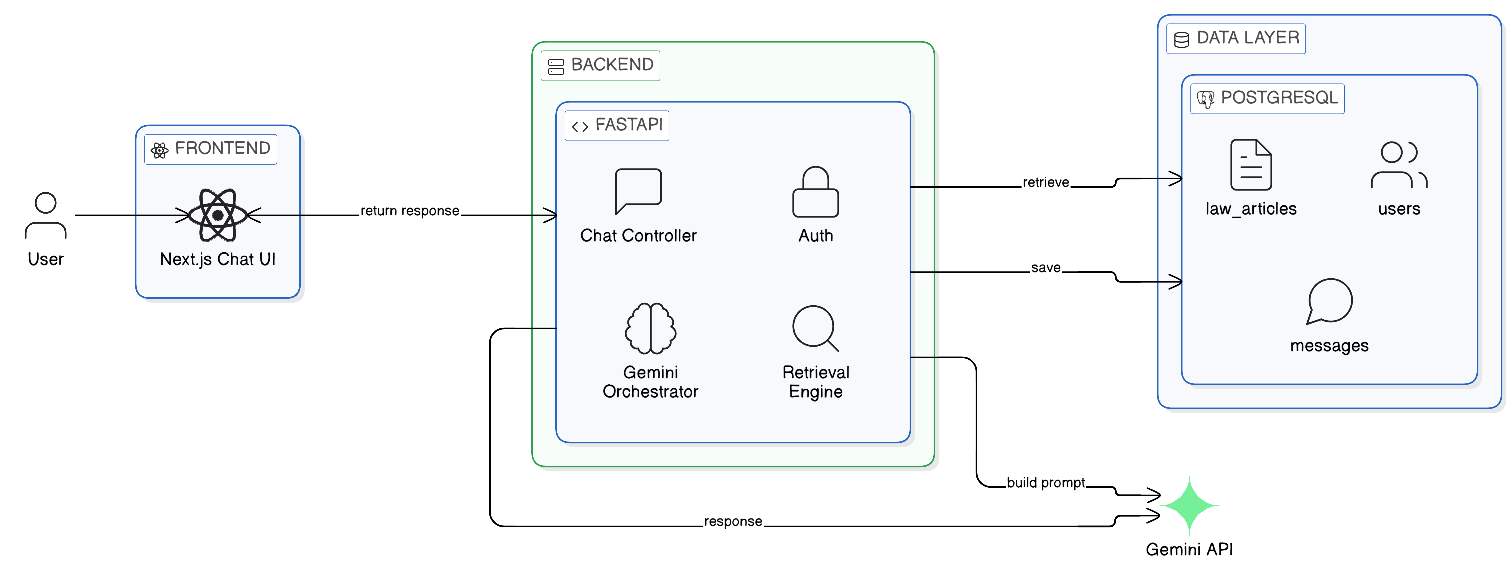
\includegraphics[width=\textwidth]{Diagrams/SystemArchitecture.png}
    \caption[Системийн ерөнхий архитектур]{Системийн ерөнхий архитектурын диаграм}
    \label{fig:SystemArchitecture}
\end{figure}

\noindent
Архитектурын диаграмм нь Frontend, Backend, Database болон AI үйлчилгээ гэсэн дөрвөн үндсэн давхаргын харилцан уялдаа, өгөгдлийн урсгалыг нэгдсэн байдлаар харуулна.

Системийн архитектур нь дараах үндсэн зарчмуудад тулгуурлана:

\begin{itemize}
    \item \textbf{Decoupling:} Frontend болон Backend хэсгүүдийг бие даасан байдлаар хөгжүүлж, REST API-аар холбосон.

    \item \textbf{Source-grounded AI processing:} AI хариуг системийн өгөгдлийн сан дахь хууль, эрх зүйн эх сурвалжид тулгуурлан RAG зарчмаар үүсгэх.

    \item \textbf{Asynchronous Processing:} FastAPI-ийн асинхрон чадварыг ашиглан олон хэрэглэгчийн хүсэлтийг зэрэг боловсруулах.

    \item \textbf{Modularity:} Системийн дотоод үйлчилгээнүүдийг тусдаа модулиар зохион байгуулж, өргөтгөх боломжийг хангах.
\end{itemize}

%-----------------------------------------

\subsection{Системийн ерөнхий архитектур (High-level)}

LexNavigator систем нь дараах гурван үндсэн давхаргаас бүрдэнэ:

\begin{enumerate}
    \item \textbf{Presentation Layer (Frontend)}

    Хэрэглэгчийн интерфэйсийг хариуцна. Хэрэглэгч асуулт оруулах, хариу харах, нэвтрэх, чат ашиглах зэрэг үйлдлийг гүйцэтгэнэ.

    \textbf{Технологи:}
    \begin{itemize}
        \item Next.js
        \item React
        \item Tailwind CSS
    \end{itemize}

    \item \textbf{Application Layer (Backend)}

    Системийн бизнес логик болон API үйлчилгээг хэрэгжүүлнэ.

    \textbf{Үндсэн үүргүүд:}
    \begin{itemize}
        \item JWT authentication хэрэгжүүлэх
        \item Хэрэглэгчийн хүсэлтийг боловсруулах
        \item RAG зарчмаар хуулийн мэдээлэл хайх
        \item Chat API боловсруулах
        \item AI үйлчилгээтэй холбогдох
    \end{itemize}

    \textbf{Технологи:}
    \begin{itemize}
        \item FastAPI
        \item Python
        \item Uvicorn
    \end{itemize}

    \item \textbf{Data \& AI Layer}

    Өгөгдөл хадгалах болон AI боловсруулалтыг хариуцна.

    \textbf{Бүрэлдэхүүн:}
    \begin{itemize}
        \item PostgreSQL (Neon) -- өгөгдлийн сан
        \item Law Articles Database -- хууль, эрх зүйн өгөгдөл
        \item Google Gemini 2.5 Flash -- AI хариу үүсгэх
    \end{itemize}
\end{enumerate}

%-----------------------------------------

\subsection{Дэлгэрэнгүй архитектур (Component-level)}

Системийн дотоод бүтэц дараах үндсэн компонентүүдээс бүрдэнэ:

\begin{itemize}

    \item \textbf{Auth Module}
    \begin{itemize}
        \item bcrypt ашиглан нууц үгийг hash хийх
        \item JWT токен үүсгэх, шалгах
        \item Хэрэглэгчийн эрхийг баталгаажуулах
    \end{itemize}

    \item \textbf{Chat Controller}
    \begin{itemize}
        \item Frontend-оос ирсэн хүсэлтийг хүлээн авах
        \item Backend доторх service-үүд рүү дамжуулах
    \end{itemize}

    \item \textbf{Legal Retrieval Engine}
    \begin{itemize}
        \item Хэрэглэгчийн асуултыг боловсруулах
        \item PostgreSQL-ээс холбогдох хууль, зүйл заалтыг хайх
        \item Олдсон мэдээллийг context болгон бэлтгэх
    \end{itemize}

    \item \textbf{Gemini Orchestrator}
    \begin{itemize}
        \item Асуулт болон хууль зүйн мэдээллийг нэгтгэх
        \item Prompt үүсгэх
        \item Gemini API руу хүсэлт илгээх
        \item Хариуг backend рүү буцаах
    \end{itemize}

    \item \textbf{Database (PostgreSQL)}
    \begin{itemize}
        \item users
        \item cases
        \item messages
        \item law\_categories
        \item law\_articles
    \end{itemize}

    \item \textbf{Data Processing Module}
    \begin{itemize}
        \item PyMuPDF ашиглан PDF задлах
        \item Regex ашиглан текст боловсруулах
        \item Хуулийг бүтэцжүүлэн хадгалах
    \end{itemize}

    \item \textbf{Logging Service}
    \begin{itemize}
        \item API хүсэлт бүртгэх
        \item Алдаа бүртгэх
        \item Чат түүх хадгалах
    \end{itemize}

\end{itemize}

%-----------------------------------------

\subsection{RAG өгөгдлийн урсгал}

RAG зарчимд суурилсан өгөгдлийн урсгалыг дараах диаграммаар харуулав.

\begin{figure}[H]
    \centering
    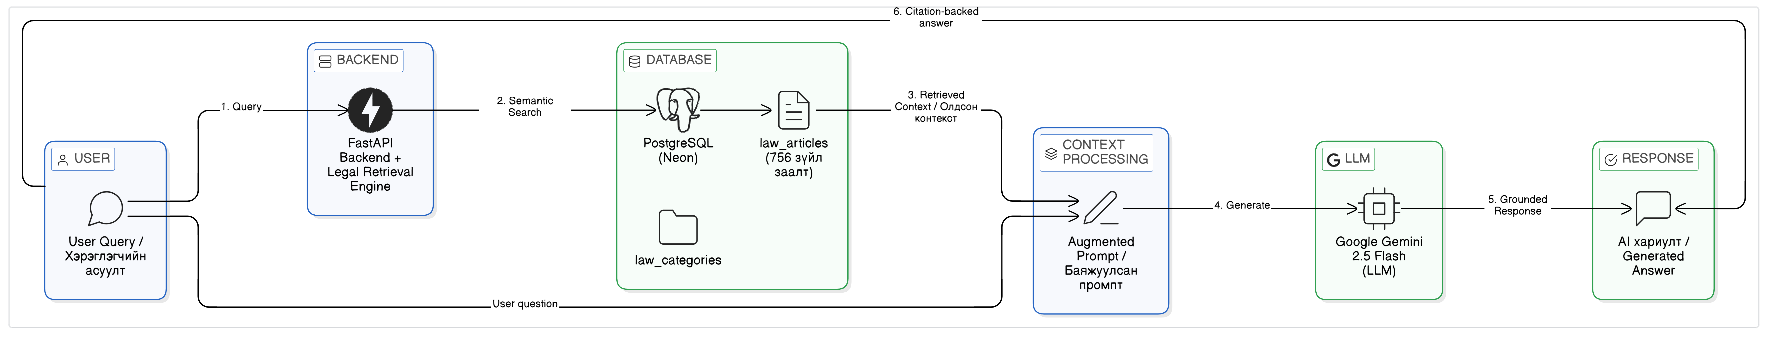
\includegraphics[width=\textwidth]{Diagrams/RAG_Diagram.png}
    \caption[RAG өгөгдлийн урсгалын диаграм]{RAG (Retrieval-Augmented Generation) өгөгдлийн урсгалын диаграм}
    \label{fig:RAGDiagram}
\end{figure}

\noindent
RAG диаграмм нь хэрэглэгчийн асуулт хүлээн авагдсанаас эхлэн өгөгдлийн сангаас холбогдох хуулийн заалтыг хайж олох (Retrieval), олдсон мэдээллийг асуулттай нэгтгэн prompt бүрдүүлэх, уг prompt-ийг Gemini загварт илгээж тайлбарласан хариулт үүсгэх (Generation) хүртэлх бүх үе шатыг нэгдсэн байдлаар харуулна.

%-----------------------------------------

\subsection{Өгөгдлийн ерөнхий урсгал (Data Flow)}

Системийн өгөгдлийн урсгал дараах байдлаар явагдана:

\begin{enumerate}
    \item Хэрэглэгч frontend дээр асуулт оруулна
    \item Frontend асуултыг backend API руу илгээнэ
    \item Backend асуултыг боловсруулж, PostgreSQL-ээс холбогдох хууль зүйн мэдээллийг RAG зарчмаар хайна
    \item Олдсон мэдээлэл болон асуултыг нэгтгэн prompt үүсгэнэ
    \item Prompt-ийг Google Gemini API руу илгээнэ
    \item AI боловсруулсан хариуг буцаана
    \item Backend хариуг хадгалж, frontend рүү дамжуулна
    \item Хэрэглэгч хариуг чат интерфейс дээр харна
\end{enumerate}

%-----------------------------------------

\subsection{Deployment архитектур}

Системийг cloud орчинд дараах байдлаар байршуулна:

\begin{itemize}
    \item Frontend -- Vercel (Next.js)
    \item Backend -- Cloud server (FastAPI + Docker)
    \item Database -- Neon PostgreSQL
    \item AI Service -- Google Gemini API
\end{itemize}

%-----------------------------------------

\subsection{Technology Stack}

\begin{table}[H]
\centering
\renewcommand{\arraystretch}{1.3}
\begin{tabular}{|p{4cm}|p{8cm}|}
\hline
\textbf{Давхарга} & \textbf{Технологи} \\ \hline
Frontend & Next.js, React, Tailwind CSS \\ \hline
Backend & FastAPI, Python, Uvicorn \\ \hline
Database & PostgreSQL (Neon) \\ \hline
AI & Google Gemini 2.5 Flash \\ \hline
Data Processing & PyMuPDF, Regex \\ \hline
Security & JWT, bcrypt \\ \hline
DevOps & Docker, GitHub \\ \hline
\end{tabular}
\caption{Системийн технологийн стек}
\end{table}

%-----------------------------------------

\subsection{Архитектурын давуу талууд}

\begin{itemize}
    \item \textbf{Өргөтгөх боломжтой:} Давхаргат бүтэц нь шинэ хууль болон функц нэмэхэд хялбар
    \item \textbf{Найдвартай байдал:} Модульчлагдсан бүтэц нь алдаа тусгаарлах боломжтой
    \item \textbf{Гүйцэтгэл сайтай:} Асинхрон backend нь олон хүсэлтийг зэрэг боловсруулах чадвартай
    \item \textbf{AI хариултын чанар:} RAG зарчмаар хууль зүйн өгөгдөлд тулгуурлан хариу үүсгэдэг тул ``hallucination'' эрсдэл буурна
    \item \textbf{Зардал хэмнэлт:} Cloud үйлчилгээ ашигласнаар дэд бүтцийн зардал буурна
    \item \textbf{Аюулгүй байдал:} JWT authentication болон password hashing ашигласан
    \item \textbf{Өгөгдөл боловсруулах чадвар:} PDF хуулийн баримтуудыг бүтэцжүүлэн ашиглах боломжтой
\end{itemize}

%-------------------------------------------------------------------------------

\section{Бүлгийн дүгнэлт}

Энэ бүлэгт хөгжүүлж буй хууль зүйн зөвлөх системийн асуудлын тодорхойлолт, хэрэглэгчийн функциональ болон функционал бус шаардлага, үндсэн оролцогч талуудын ашиглалтын хувилбаруудыг тодорхойллоо. Мөн юзкейс, нэвтрэлт болон чатын үйл ажиллагааны диаграм, дарааллын диаграм, хамаарлын диаграм, класс диаграмаар дамжуулан системийн бүтэц, ажиллагааны логик, өгөгдлийн уялдаа холбоог загварчилсан. Системийн архитектур нь RAG зарчимд тулгуурлан хуулийн өгөгдөлд суурилсан хариулт боловсруулдаг тул зөвхөн эрүүгийн хуульд бус, төрөл бүрийн хууль, эрх зүйн эх сурвалжид тулгуурлан хэрэглэгчид бүрэн хэмжээний хууль зүйн зөвлөгөө өгөх боломжтой цогц систем юм.